\documentclass[tikz,border=8pt]{standalone}
% Shared look for every TikZ diagram. Load with \input{../../tools/tikz-style.tex}
\usepackage[T1]{fontenc}
\usepackage{lmodern}
\renewcommand{\sfdefault}{lmr}  % diagrams use the same serif as the text
\usetikzlibrary{arrows.meta, positioning, shapes.geometric, calc, fit, backgrounds}
\definecolor{cblue}{HTML}{4C78A8}
\definecolor{corange}{HTML}{F58518}
\definecolor{cgreen}{HTML}{54A24B}
\definecolor{cred}{HTML}{E45756}
\definecolor{cpurple}{HTML}{B279A2}
\definecolor{cgrey}{HTML}{6B6B6B}
\tikzset{
  every picture/.style={font=\sffamily, line width=1.2pt},
  box/.style={draw=#1, fill=#1!12, rounded corners=4pt, align=center, inner sep=7pt, minimum height=1.1cm},
  box/.default=cgrey,
  arrow/.style={-{Stealth[length=3mm]}, draw=cgrey, line width=1.4pt},
  title/.style={font=\sffamily\bfseries\Large},
  note/.style={font=\sffamily\small, text=cgrey, align=center},
}
\AtBeginDocument{\hyphenpenalty=10000 \exhyphenpenalty=10000}

\begin{document}
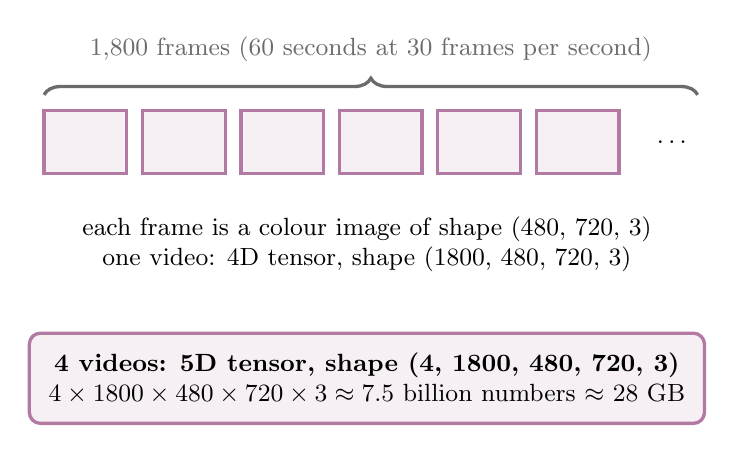
\begin{tikzpicture}
  \foreach \f in {0,...,5}
    \filldraw[draw=cpurple, fill=cpurple!12] (\f*1.25,0) rectangle ++(1.05,0.8);
  \node[font=\small] at (8.0,0.4) {\dots};
  \draw[decorate, decoration={brace, amplitude=6pt}, cgrey] (0,1.0) -- (8.3,1.0) node[midway, above=8pt, font=\small] {1,800 frames (60 seconds at 30 frames per second)};
  \node[align=center, font=\small] at (4.1,-0.9) {each frame is a colour image of shape (480, 720, 3)\\one video: 4D tensor, shape (1800, 480, 720, 3)};
  \node[box=cpurple, align=center, font=\small] at (4.1,-2.6) {\textbf{4 videos: 5D tensor, shape (4, 1800, 480, 720, 3)}\\$4 \times 1800 \times 480 \times 720 \times 3 \approx 7.5$ billion numbers $\approx$ 28 GB};
\end{tikzpicture}
\end{document}
